\documentclass[12pt,a4paper]{article}

% ---------------------
% Packages
% ---------------------
% \usepackage[utf8]{inputenc}   % encoding
\usepackage[T1]{fontenc}      % font encoding
\usepackage{lmodern}          % clean font

\usepackage{geometry}         % page margins
\geometry{margin=1in}

\usepackage{amsmath, amssymb, amsthm}  % math
\usepackage{mathtools}                  

\usepackage{hyperref}         % hyperlinks
\hypersetup{
    colorlinks=true,
    linkcolor=blue,
    urlcolor=cyan
}

\usepackage{graphicx}         % images
\usepackage{float}           
\usepackage{caption}          % in preamble

\usepackage{xcolor}           % colored text

\usepackage{listings}         % code snippets
\usepackage{courier}          % monospace font for code

\usepackage{enumitem}         % customize lists
\setlist{nosep}               % no extra space in lists
\setlength{\parskip}{1em}

% ---------------------
% Code snippet settings
% ---------------------
\lstset{
    language=C++,
    basicstyle=\footnotesize\ttfamily,
    keywordstyle=\color{blue},
    commentstyle=\color{green!60!black},
    stringstyle=\color{red!80!black},
    % numbers=left,
    % numberstyle=\tiny,
    frame=single,
    breaklines=true,
    captionpos=b,
    tabsize=4,
    xleftmargin=2em,
    xrightmargin=2em,
    aboveskip=1em
}

% ---------------------
% Theorem-like environments
% ---------------------
\newtheorem{theorem}{Theorem}[section]
\newtheorem{lemma}[theorem]{Lemma}
\newtheorem{definition}[theorem]{Definition}
\newtheorem{example}[theorem]{Example}

% ---------------------
% Custom commands
% ---------------------
\newcommand{\code}[1]{\texttt{#1}}
\newcommand{\ds}{\displaystyle}

% ---------------------
% Document
% ---------------------
\begin{document}
\title{Competitive Programming Notes}
\author{Pakin Olanraktham}
\date{\today}

\maketitle

\newpage

\tableofcontents
\newpage

% ---------------------

\section{Range Query}
\subsection{Segment Tree}

\section{Dynamic Programming Optimization}
\subsection{Convex Hull Trick}

Convex Hull Trick is an algorithm to find $\min_{j < i}(f_j(x))$ or $\max_{j < i}(f_j(x))$ efficiently.

First, we convert the function $f(x)$ to $mx+c$, which $x$ depends only on $i$, $m$ and $c$ depends only on $j$. For example

\begin{lstlisting}
dp[i] = max(dp[j] + x[i]*y[i] - x[j]*y[i] - a[i])
      = max((-x[j])*y[i] + dp[j]) + x[i]*y[i] - a[i]
\end{lstlisting}

As we can see, m = -x[j], x = y[i], c = dp[j]. Note that if we want to do CHT, the slope \textbf{must} be monotonic. Otherwise, we have to use Li Chao Tree.

Now, how do we compute the maximum or minimum? We know that the recurrence is a line with monotonic slope.

\subsubsection{Inserting}

We will use \texttt{deque <int>} to store the lines indices.

For computing maximum, we want to maintain the lines as lower hull shaped. For minimum, we want the lines as upper hull shaped.

Before inserting, we have to check whether the old line is useless or not. We can do that by checking the intersection point between the [new line, top] and [top, top-1]. (You should try drawing on paper by yourself.)

\begin{figure}[h]
    \centering
    \begin{minipage}{0.4\textwidth}
        \centering
        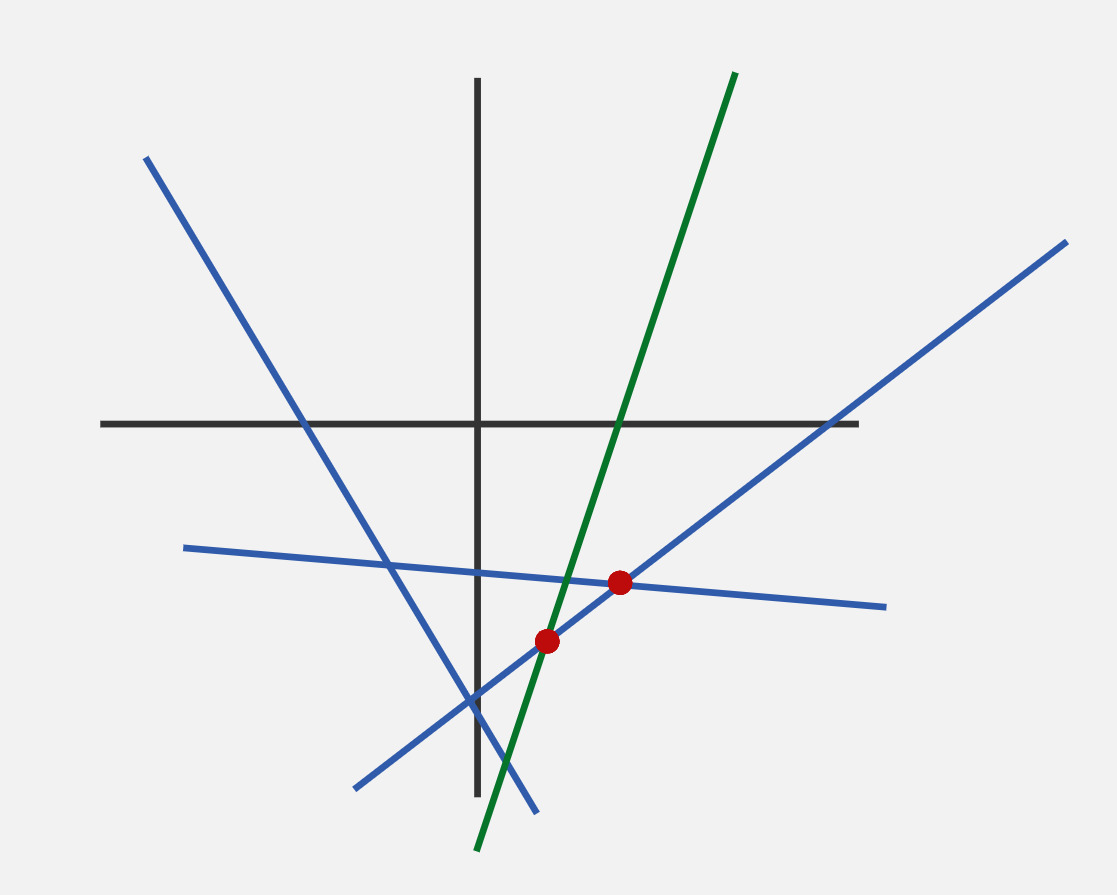
\includegraphics[width=\textwidth]{assets/cht_max.jpg}
        \caption*{Lower Hull (Maximum)}
    \end{minipage}
    \hfill
    \begin{minipage}{0.4\textwidth}
        \centering
        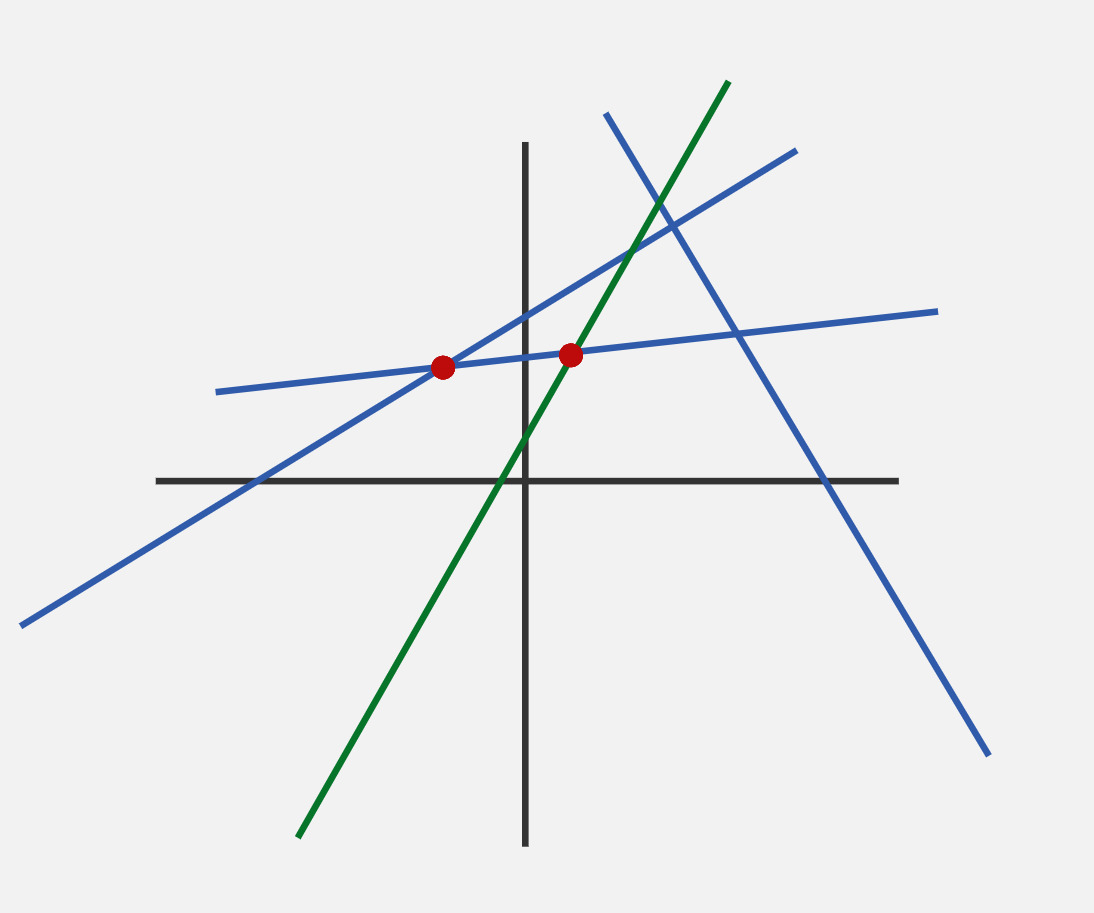
\includegraphics[width=\textwidth]{assets/cht_min.jpg}
        \caption*{Upper Hull (Minimum)}
    \end{minipage}
\end{figure}

For finding the intersection point we can do

\begin{lstlisting}
double m(int x, int y) {
    return (double) (c[x] - c[y]) / (m[y] - m[x]);
}
\end{lstlisting}

\subsubsection{Querying}

\textbf{Monotone Query}

If the hull is maintained correctly for each type of query, we will always query from front for non-decreasing queries, and always from back for non-increasing queries.

We will check the top and top-1. For maximum, if $f_\text{top}(x) \le f_\text{top-1}(x)$, we pop the top. For minimum, if $f_\text{top}(x) \ge f_{\text{top-1}}(x)$, we pop the top. For example

\begin{lstlisting}
while (sz > 1 && calc(cht[0], p[i]) <= calc(cht[1], p[i])) {
    cht.pop_front(), sz--;
}
\end{lstlisting}

Then the answer will be $f_\text{top}(x) + c$ where $c$ is a constant that depends only on $x$.

\noindent\textbf{Arbitrary Query}

We perform a binary search for the line that contain $x$.

\begin{figure}[h]
    \centering
    \centering
    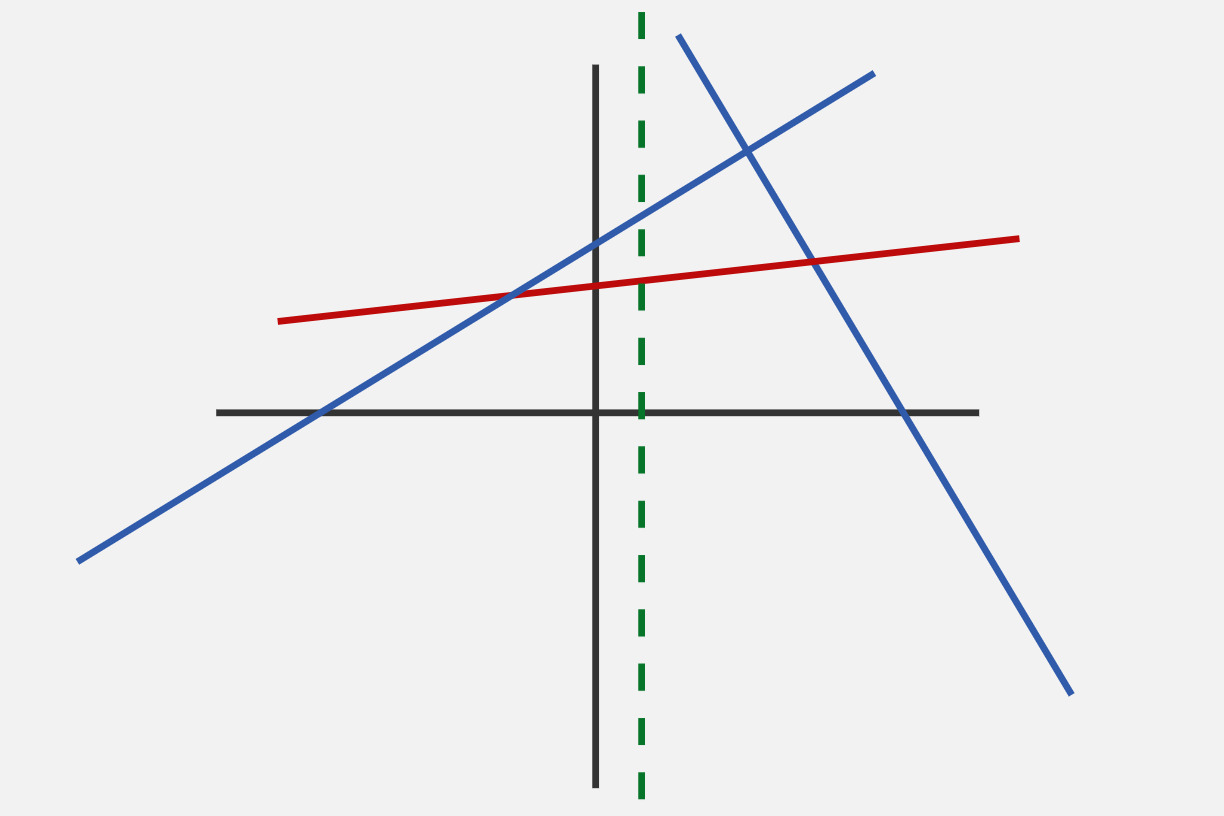
\includegraphics[width=0.6\textwidth]{assets/cht_qry.jpg}
\end{figure}

\begin{lstlisting}
int l = 0, r = sz-2, idx = sz-1;
while (l <= r) {
    int mid = l + (r-l)/2;
    if (m(cht[mid], cht[mid+1]) <= x) l = mid+1;
    else r = mid-1, idx = mid;
}
\end{lstlisting}

\break

\section{Tree Algorithms}
\subsection{Centroid Decomposition}
\subsubsection{Centroid}
A centroid of a tree is defined as a node such that if removed, no connected component has  more than $\frac{N}{2}$ nodes.

We can find a centroid in a tree by selecting an arbitrary node in the tree. Then loop through its children's subtree. If the size of a child's subtree is more than $\frac{N}{2}$, traverse down that node. Otherwise, if no child's subtree has size more than $\frac{N}{2}$, then that node is the centroid.

\begin{lstlisting}
void fsz(int u, int p) {
    sz[u] = 1;
    for (auto v : adj[u]) if (v != p) fsz(v, u), sz[u] += sz[v];
}

int ct(int u, int p) {
    for (auto v : adj[u]) if (sz[v] * 2 > n) return ct(v, u);
    return u;
}
\end{lstlisting}

\noindent\textbf{Properties}
\begin{enumerate}
    \item If the centroid of a tree isn't unique, there are exactly two centroids which are adjacent. Removing the edge between them divides the tree into two connected components of the equal sizes.
    \item When a leaf is added to or removed from a tree, the centroid changes by at most one node.
    \item When two trees are connected, the centroid of the resulting tree lies on the path between the centroids of the original trees.
\end{enumerate}

\subsubsection{Centroid Decomposition}

Centroid Decomposition is a divide-and-conquer technique for trees, which recursively splits the tree by removing its centroid. The resulting decomposition tree has a height of at most $\mathcal{O}(\log N)$.

\noindent\textbf{Properties}
\begin{enumerate}
    \item The height of the decomposed tree is at most $\log{N}$
    \item Every path between $u$ and $v$ can be decomposed into two parts: $u$ to $\text{lca}_{ctd}(u, v)$ and $\text{lca}_{ctd}(u, v)$ to $v$. We can use this property for querying and updating. In the \textbf{Xania and Tree} problem, we update and query by traversing up to the $\log{N}$ parents for each node.
\end{enumerate}

\begin{lstlisting}
int fsz(int u, int p) {
    sz[u] = 1;
    for (auto v : adj[u]) if (v != p && !vis[v]) sz[u] += fsz(v, u);
    return sz[u];
}
 
int ct(int u, int p, int tsz) {
    for (auto v : adj[u]) if (v != p && !vis[v]) if (sz[v] * 2 > tsz) return ct(v, u, tsz);
    return u;
}
 
void ctd(int u, int p) {
    int C = ct(u, u, fsz(u, u));
    vis[C] = 1;
    if (p == -1) p = C;
    par[C] = p;
    for (auto v : adj[C]) if (!vis[v]) ctd(v, C);
}
\end{lstlisting}

\end{document}